\documentclass[a4paper,11pt]{article}
\usepackage[utf8]{inputenc}
\usepackage[OT1]{fontenc}
\usepackage[english]{babel}
\usepackage[margin=1.2in]{geometry}
\usepackage{graphicx}
\usepackage{amsmath}
\usepackage{cite}
\usepackage[perpage,symbol]{footmisc}
\usepackage[hang,small]{caption}
\usepackage{parskip}
\usepackage{array}
\usepackage{pstricks}
\usepackage{hyperref}
%\usepackage{pslatex}

\usepackage{fancyvrb}

\author{Simon Mitternacht} 
\date{\today} 
\title{FreeSASA: A Free C Library for Solvent Accessible Surface
  Area Calculations
}
\begin{document}
\maketitle

%\hrule
\subsection*{Abstract}
FreeSASA is a C library, and command line tool, for calculating
Solvent Accessible Surface Area (SASA), released under the GNU General
Public License 3\footnote{See
  \url{http://www.gnu.org/licenses/gpl.html}}. It implements the
classic algorithms by Lee and Richards and by Shrake and Rupley. The
source code is freely available at
\url{https://github.com/mittinatten/freesasa/}.  The functionality is
not new, but to the author's knowledge this is the only available tool
released under an open source license.

\section{Introduction}
The Solvent Accessible Surface Area (SASA) of a molecule gives a
measure of the contact area between molecule and solvent. This
area can for example quantify how folded the conformation of a
macromolecule is, and can also be used to compare the exposed
hydrophobic surfaces of different conformations or different
molecules. To define the SASA, $A$, of a given molecule, let a
spherical probe roll over the surface of the molecule, including
internal cavities. $A$ is then the surface drawn by the center of the
probe.~\cite{LnR} The probe represents a solvent molecule
(i.e.\ water). Cavities smaller than the solvent molecule do not
contribute to $A$.

Calculating Solvent Accessible Surface Areas (SASA) is a
run-of-the-mill calculation in protein structure studies. To the
author's knowledge there are no fully open source standalone programs
for doing this. Neither are there any libraries designed to be easily
integrated in other programs. The present library is an attempt to
resolve both these issues, and is released under the GNU General
Public License 3.

FreeSASA is a both a standalone command line program and a C library
for protein SASA calculations. The library provides a simple interface
that takes PDB-files as input. It has default parameters to allow
straightforward calculations, but also allows the user to change most
parameters of the calculation. In addition, the user can treat the
calculation as a purely mathematical operation on a set of spheres, by
providing arbitrary coordinates and radii. Both Lee \& Richards'
\cite{LnR} and Shrake \& Rupley's \cite{SnR} algorithms are
available. They will be referred to as L\&R and S\&R throughout this
document. Future versions of the library might include other
algorithms as well. In the current implementation S\&R is the more
effecient, and therefore recommended for most applications.

In constructing the library three possible use cases were considered. 
\begin{enumerate}
\item The user has a PDB-file and wishes to calculate the total SASA of
  the structure, or the SASA for certain groups or types of atoms.
\item The user has a set of spheres (typically a molecule), and wants
  to calculate the total SASA for this object.
\item The user is simulating different conformations of a molecule and
  wants to measure the SASA at certain intervals during the simulation.
\end{enumerate}
For case 1 both the command-line interface (CLI) and the application
programming interface (API) can be used. Using the API gives more
flexibility in interpreting and analyzing the results. The other 2
cases can only be handled through the API. Both the API and the CLI
allow the user to set parameters for the calculation. 

This document is organized as follows. Section \ref{sec:howto_short}
gives a brief introduction to the library, presenting the command line
interface and a short sample program that gives a general idea of how
to use the library. The introduction is intended to cover most casual
users' needs. Section \ref{sec:using} gives a detailed description of
the API. Appendix \ref{sec:alg} describes the algorithms, appendix
\ref{sec:imp} their implementation. Appendix \ref{sec:compare}
compares their performance in terms of computational cost and
precision.

\section{Getting started}\label{sec:howto_short}

The source files \verb|main.c| and \verb|example.c| contain
a complete command-line interface and a minimal program to illustrate
how to use the library interface, respectively. 

\subsection{Installation} \label{sec:installing}

The repository can be cloned from github, either by using git directly
with the command
\begin{verbatim}
    $ git clone https://github.com/mittinatten/freesasa.git
\end{verbatim}
or by downloading the zipped archive from
\begin{verbatim}
    https://github.com/mittinatten/freesasa/archive/master.zip
\end{verbatim}
FreeSASA itself only depends on regular C and GNU libraries, and
should therefore be straightforward to compile and
install. Installation is done by the regular sequence
\verb|./configure|, \verb|make| and \verb|make install|. Several
versions of the GNU C Compiler and Clang/LLVM have been tested
successfully on both Linux and Mac OS X platforms. The test-suite
depends on the Check unit testing
framework\footnote{\texttt{http://check.sourceforge.net/}} (not
necessary to build the program itself). Doxygen is required to build
the full html reference manual.

\subsection{Command-line interface}

Compilation creates the binary \verb|freesasa| from
\verb|main.c|, which can be used to calculate the SASA of a
PDB-file. The simplest program call, with default parameters would be
\begin{verbatim}
    $ freesasa PDB-file
\end{verbatim}
Or, from \verb|stdin|:
\begin{verbatim} 
    $ freesasa < PDB-file    
\end{verbatim}
\verb|stdin| is only read if no file is specified.  By default the
Shrake \& Rupley algorithm is used, with 100 test points. Running the
program using the default parameters on the PDB structure 1UBQ gives
the following output
\begin{verbatim}
   name: 1ubq.pdb
   algorithm: Shrake & Rupley
   probe-radius: 1.400000 A
   n_thread: 1
   n_testpoint: 100
   
   Total:    4756.12 A2
   Polar:    1968.06 A2
   Apolar:   2788.07 A2
\end{verbatim}
The first 5 lines contain info about input and parameters. This is
followed by data for calculation time and the size of the
protein. Finally the result of the calculation is printed, with SASA
values in Å$^2$.

As an illustration of a few of the configuration options, the command
\begin{verbatim}
   $ freesasa -L -d 0.1 -B -l PDB-file
\end{verbatim}
calculates the SASA of the supplied PDB-file using Lee \& Richards
(-L), with a slice width of 0.1 Å (-d). The option -l suppresses the
regular log message. Output will instead, beacuse of the flag -B, be
the provided PDB-file with the SASA of each atom replacing the
temperature factors, and the atomic radii stored in the occupancy
factor field, written to \verb|stdout|. The program can thus be used
as a PDB-file filter. If a file-name is provided after -B the
output will be written to that file instead.

The command \verb|freesasa -h| prints a help message listing all
available options. The program classifies each atom and assigns it an
atomic radius accordingly, based on the PDB input, but users can also
provide their own configuration files to customize classification (via
-c).  Several PDB-files can be analyzed in one call, the results will
be printed consecutively for each input file:
\begin{verbatim}
   $ freesasa 1abc.pdb 2abc.pdb ...
\end{verbatim}
If several threads are requested each calculation is parallelized
individually, if the user wants to analyze several proteins
simultaneously this will have to be done by calling several instances
of the program.

\subsection{Application programming interface}\label{sec:api}

As an illustration of the API, figure~\ref{fig:example_c} shows the
minimal program \verb|example.c|, which performs a SASA-calculation
using a PDB-file as input, with no error handling and default
parameters. The three points were null pointers are passed as
arguments are places were user-defined parameters and atomic
classifiers could have been provided. The source code for the CLI, in
the file \verb|main.c|, illustrates full-fledged use of most parts of
the API including error checking and customization. The example here
is meant to illustrate the most basic parts of the library interface
and is by default compiled to a binary called \verb|example| using
\verb|make|.

\begin{figure}
  \begin{Verbatim}[frame=single,fontsize=\small,framesep=5mm]
// example.c
#include <stdlib.h>
#include <stdio.h>
#include "freesasa.h"

int main(int argc, char **argv) {
    freesasa_result* result;
    freesasa_strvp *class_area;
    freesasa_structure *structure;
    double *radii;

    // Read structure from stdin
    structure = freesasa_structure_from_pdb(stdin,0);

    // Calculate radii for the atoms
    radii = freesasa_structure_radius(structure,NULL);

    // Calculate SASA using structure and radii, store in 'result'
    result = freesasa_calc_structure(structure,radii,NULL);
    
    // Calculate area of classe (Polar/Apolar/..)
    class_area = freesasa_result_classify(result,structure,NULL);

    // Print results
    printf("Total area: %f A2\n",result->total);
    for (int i = 0; i < class_area->n; ++i)
        printf("%s: %f A2\n",class_area->string[i],class_area->value[i]);

    // Free allocated resources, not strictly necessary but good style
    freesasa_result_free(result);
    freesasa_strvp_free(class_area);
    freesasa_structure_free(structure);
    free(radii);

    return EXIT_SUCCESS;
}
  \end{Verbatim}
  \caption{An example program demonstrating basic use of the
    library. No error checks are done here. \label{fig:example_c}}
\end{figure}

This program generates output similar to that of the previous
section.

\appendix

\begin{small}

\section{Algorithms}\label{sec:alg}

There are two classical approximate algorithms that can be used to
calculate SASA. One by Lee \& Richards \cite{LnR} where the surface is
calculated for slices of the protein and then added up, one by Shrake
\& Rupley \cite{SnR} where the surface of each sphere is approximated
by a set of test points. The SASA can be calculated to arbitrary
precision by refining the resolution of both. 

As will be clear from this section and the analysis in section
\ref{sec:compare}, S\&R is the simpler and faster of the
two. Therefore the casual user is recommended to use S\&R. L\&R is
mainly included for reference, and for the fact that the precision is
only limited by floating point precision. In the current
implementation S\&R can only be used with a predefined set of levels
of precision. However, it is not obvious what applications would
require very high precision SASA values.

We will use the following notation: An atom $i$ has a van der Waals
radius $r_i$, the rolling sphere (or \emph{probe}) has radius
$r_\text{P}$ and when these are added we get an extended radius $R_i =
r_i + r_\text{P}$. The sphere of radius $R_i$ centered at the position
of atom $i$ represents the volume not accessible to the center of the
probe. The SASA for a molecule is then obtained by calculating the
non-buried surface area of the extended spheres.

\subsection{L\&R} \label{sec:alg_LnR}

Lee \& Richards' algorithm calculates the surface area by slicing the
protein, calculating the length of the solvent exposed contours in
each slice and then adding up the length multiplied by the slice
thickness. Precision is increased by making the slices thinner and the
calculation time scales approximately as the number of slices.

Divide the protein into slices of thickness $\delta$ along an
arbitrary axis. The position of the middle of the slice along that
axis is denoted $z$, as in figure~\ref{fig:slice}. The center of atom
$i$, along the same axis, is at $z_i$. In the slice, each atom is thus
a circle of radius $$R_i^\prime = \sqrt{R_i^2-(z-z_i)^2}\,.$$ These
circles are either completely buried, completely exposed, or partially
exposed.

\begin{figure}
%\begin{center}
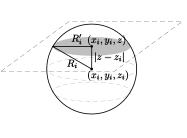
\includegraphics{fig/lnr_slice}

\includegraphics{fig/lnr_circles}
\caption{Geometry of slice in L\&R.\label{fig:slice}}
\end{figure}

The exposed arc lengths for each atom can be calculated exactly. For
each pair of atoms $i,j$, the distance between their centers projected
on the slice is $d_{ij}$ (independent of $z$). If $d_{ij} > R_i^\prime
+ R_j^\prime$, there is no overlap. If $d_{ij} < R_j^\prime -
R_i^\prime$ circle $i$ is completely inside $j$ (and the other way
around). If $d_{ij}$ lies between these two cases the angle of circle
$i$ that is buried due to circle $j$ is $$\alpha = 2\arccos
\bigl[({R_i^\prime}^2 + d_{ij}^2 - {R_{j}^\prime}^2)/(2R_i^\prime
  d_{ij})\bigr].$$ The middle point of the arc on the circle is at an
angle $\beta$ in circle $i$, and thus the arc spans the interval
$[\beta-\alpha/2,\beta+\alpha/2]$ on the circle. By adding up these
arcs and taking into account any overlap between them we get the total
buried angle $\gamma_i$ of circle $i$. The exposed arc length in this
slice is thus $L_i = R_i^\prime(2\pi-\gamma_i)$.

The contribution to the SASA from each slice is $$ S_\delta =
\sum_{i \in \text{slice}}L_i\Delta_i $$ where
$$
  \Delta_i = \frac{R_i}{R_i^\prime} \biggl[\frac{\delta}{2} 
    + \min\biggl(\frac{\delta}{2},R_i -
    \lvert z - z_i \rvert\biggr)\biggr]. 
$$ 
The factor $R_i/R_i^\prime$ comes from approximating the area of the
slice by a conical segment of the sphere, instead of a cylinder.
Finally, the total SASA is obtained by adding up the contribution from
all the slices, either for the whole protein, or atom by atom.

\subsection{S\&R}

Shrake \& Rupley's algorithm uses test points on a sphere to estimate
what parts of an atom are exposed. For each atom $i$, use a set of
test points evenly distributed (approximately) over the sphere of
radius $R_i$, and count how many of the test points are not inside any
other sphere. The number of exposed test points divided by the total
number of test points gives the exposed solid angle of that atom. The
precision of the algorithm is increased by increasing the number of
test points, and calculation time scales approximately linearly with
the number of test points.

\section{Implementation}\label{sec:imp}

The correctness of the implementations was tested by comparing with
analytical results for the two atom case, and by performing high
precision SASA calculations using the two independent algorithms for a
large number of proteins (see section \ref{sec:dataset}) and comparing
the results. In addition, the calculated surface test
points and slice contours were inspected visually.

Both algorithms require determining which atoms are in contact, this
is done by Verlet lists~\cite{Verlet}, which means the calculation
time is $O(N)$. There is a slight overhead in generating the lists,
which means that for small proteins the calculations are slower than
in a na\"{i}ve $O(N^2)$ implementation. The gains are however
significant for large proteins.

\subsection{L\&R}

In FreeSASA, the L\&R SASA calculation begins by finding overlapping
spheres and storing the contacts in an adjacency list. For a given
slice, one needs then only check the overlap between circles that are
in the slice, and are known to potentially be in contact. The buried
arcs due to overlapping circles are calculated as described in section
\ref{sec:alg_LnR}. When all buried arcs have been counted for a given
circle they are reduced to non-overlapping intervals recursively. In
most cases only one recursion step is necessary. The lengths of
exposed arcs are then summed up for all atoms in the slice to
calculate the total contribution to the area as described in
\ref{sec:alg_LnR}.

As we will see in section \ref{sec:accuracy}, this algorithm is
significantly slower than S\&R. Profiling runs give no hints at
obvious improvements. The calculations of each slice are completely
independent and the current implementation allows division of labor to
an arbitrary number of threads, whereas the calculation of adjacency
lists has not been parallelized.

\subsection{S\&R}

Test points were generated by placing a given number of equally
charged particles on the surface of a sphere and then minimizing the
Coulomb potential using a simple Monte Carlo simulation. The obtained
sets of test-points are then stored as static arrays in a special
source file (\texttt{srp.c}), to make the program independent of any
auxiliary input files. Sets containing 20, 50, 100, 200, 500, 1000,
2000 and 5000 test points are included in the program. This set should
cover most users' need for speed and accuracy.

\section{Comparison of the two}\label{sec:compare}

[The data in this section corresponds to an older version of the code
  without Verlet lists.]

\subsection{Data set}\label{sec:dataset}

For evaluating and comparing the two algorithms a list of proteins was
downloaded from the PISCES server \cite{PISCES} (on Aug 12, 2013). The
proteins have less than 20\,\% sequence identity, and the structures a
resolution of 1.6~Å or less and R-factors less than 0.25\footnote{The
  resolution of the structures is not relevant for the present
  study. It was only restricted to get a sufficiently small set of
  independent structures.}. The list specifies which chain to use in a
specific PDB-file. For the calculations here, whole PDB-files are
used, giving a larger variation in protein size, which is useful for
our purposes. The 2117 chains in the list gave a set of 2056 protein
structures used for all calculations below.

\subsection{Speed}\label{sec:speed}

In the limit of low precision the calculation time will be limited by
the time it takes to find which atoms are neighbors, which scales as
the square of the number of atoms. As described above this calculation
can be linearized, but with a relatively large overhead making it
worthwhile only for large proteins.

In the limit of high precision the calculation time of both algorithms
will instead scale as the number of atoms: If the number of
test-points is large in S\&R, most of the time will be spent
calculating the extent of overlap, instead of which atoms are in
contact. If there are many slices in L\&R, the calculation time will
be proportional to the number of slices, and the time of each slice
linear in the number of atoms in the slice.  The point where the
calculation time crosses over from linear to quadratic in the number
of atoms thus depends on the precision as figure~\ref{fig:time} shows.

\begin{figure}
  \begin{center}
  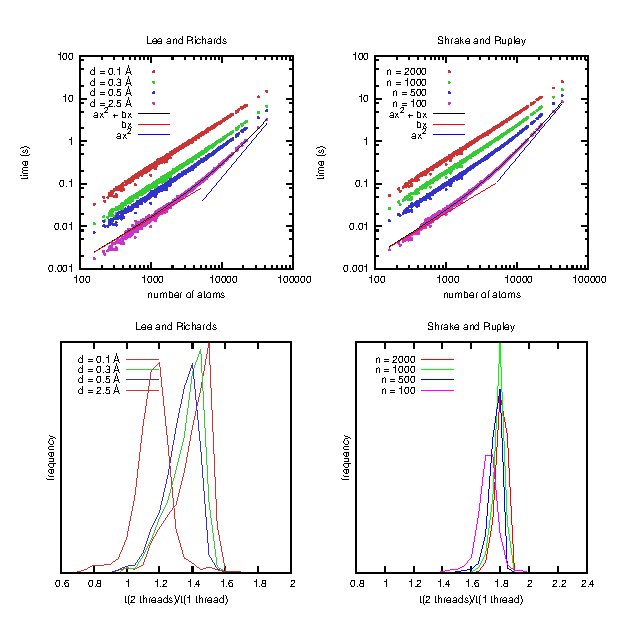
\includegraphics{fig/time}
  \caption{(Top) Calculation time as function of number of atoms for
    different levels of precision. In both cases the cross-over from
    linear to quadratic scaling as function of protein size is only
    clearly visible for the lowest precision used.  (Bottom)
    Comparison of calculation time with one and two threads, the
    histograms shows the distribution of the calculation time using
    two threads divided by the time using one thread. Thus a value of
    2 would correspond to ``perfect'' parallelization. The values
    above 2 are likely due to noise, i.e. in the very short
    simulations the timing is both inexact and might be affected by
    random factors such as background system processes.
    \label{fig:time}}
  \end{center}
\end{figure}

Where it can be done trivially, both algorithms have been
parallelized in FreeSASA. As mentioned above, in S\&R each atom can be treated
independently, and in L\&R each slice. The efficiency of the
parallelization in a two-threaded run can be seen in figure
\ref{fig:time}. For S\&R the speed increase is close to twofold and
almost independent of the accuracy, as expected. For L\&R the
efficiency of parallelization increases with precision, i.e. the more
slices are calculated, the more there is to gain from parallelizing
the calculations. This result was also expected since the time needed
to compute which atoms are neighbors, which is done in only one thread
in the current implement, is independent of precision.

\subsection{Accuracy as function of speed}\label{sec:accuracy}

To measure accuracy of the two algorithms a reference SASA value,
$S_\text{ref}$ was calculated using L\&R with slice thickness
0.001~Å. The error of a given SASA-value, $S$ is then $\delta = \lvert
S - S_\text{ref} \rvert / N$, where $N$ is the number of atoms in the
protein. Figure~\ref{fig:precision} shows the results of these
calculations for the 2056 proteins described above.  It is clear from
this picture that S\&R is on average an order of magnitude more
accurate than L\&R given the same computational effort -- in the
present implementation.

\begin{figure}
  \begin{center}
  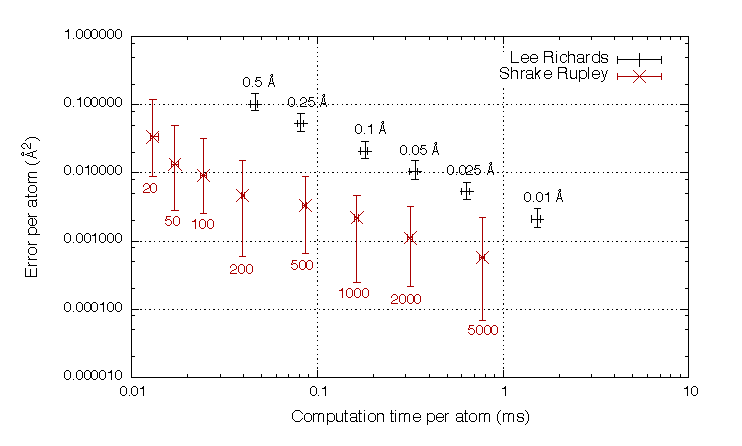
\includegraphics{fig/precision}
  \caption{The error $\delta$ in calculated SASA vs calculation time
    $t$ for the two algorithms. For the different S\&R calculations
    20, 50, 100, 200, 500, 1000, 2000 and 5000 test points were
    used. For L\&R slice thicknesses 0.01, 0.1, 0.2, 0.3, 0.5, 1.0,
    2.5 and 5.0 Å. The borders of the boxes indicate the quartiles of
    the distribution of $t$ and $\delta$ (i.e. 50~\% of the data are
    within the box), and the error bars 5th and 95th percentiles.  The
    horizontal bars are wider for S\&R because calculation time is
    less linear as function of the number of atoms than for L\&R (see
    figure~\ref{fig:time}). It is not clear why the precision varies
    more for S\&R than for L\&R.
    \label{fig:precision}}
  \end{center}
\end{figure}

\end{small}

\begin{thebibliography}{50}

\bibitem{LnR} 
  Lee B, Richards FM (1971) The interpretation of protein
  structures: estimation of static accessibility. Journal of molecular
  biology 55: 379–-400.

\bibitem{SnR} 
  Shrake A, Rupley JA (1973) Environment and exposure to
  solvent of protein atoms. Lysozyme and insulin. Journal of Molecular
  Biology 79: 351–-371.

\bibitem{OONS} 
  Ooi T, Oobatake M, Némethy G, Scheraga H (1987)
  Accessible surface areas as a measure of the thermodynamic
  parameters of hydration of peptides. Proceedings of the National
  Academy of Sciences of the United States of America 84: 3086–3090.

\bibitem{Verlet} 
  Verlet, L (1967). Computer ``Experiments'' on Classical
  Fluids. I. Thermodynamical Properties of Lennard-Jones
  Molecules. Physical Review 159: 98--103.

\bibitem{PISCES}
  Wang G, Dunbrack RL (2003) PISCES: a protein sequence culling server. 
  Bioinformatics 19:1589--1591.

\end{thebibliography}

\end{document}
